\documentclass[a4paper,11pt]{article}
  \usepackage[T1]{fontenc}
  \usepackage[utf8]{inputenc}
  \usepackage[italian]{babel}
  \usepackage{tabularx}
  \usepackage[font=small,labelfont=bf]{caption}
  \usepackage[footskip=0.4in]{geometry}
  \usepackage{enumitem}
  \usepackage{graphicx}
  \usepackage{amssymb}
  \usepackage{wrapfig}
  \usepackage{tgcursor}
  \usepackage[dvipsnames]{xcolor}
  \usepackage{listings}
  \usepackage{fancyvrb}
  \usepackage{color}
  \usepackage{mathtools}
  \usepackage{nameref}
  \usepackage{array,collcell}
  \usepackage{tikz}
  \usepackage{tikz-qtree}
  \usepackage{float}
  \usepackage{subfig}
  \usepackage{csquotes} % Quotes
  \usepackage{booktabs} % For \toprule, \midrule and \bottomrule
  \usepackage{siunitx} % Formats the units and values
  \usepackage{pgfplotstable} % Generates table from .csv
  \usepackage{hyperref}
  \usepackage{caption}
  \usepackage{longtable}
  \usepackage{amssymb}

  \captionsetup[table]{position=bottom}

  % Setup siunitx:
  \sisetup{
    round-mode          = places, % Rounds numbers
    round-precision     = 2, % to 2 places
  }

  % Setup hyperref
  \hypersetup{
    colorlinks=true,
    linkcolor=NavyBlue,
    filecolor=magenta,
    urlcolor=cyan,
    pdftitle={Algoritmi Avanzati - Laboratorio 1},
    bookmarks=true,
    pdfpagemode=FullScreen,
  }

  % \usepackage{amsmath}
  \DefineShortVerb{\|}
  \fontfamily{arial}

   % C++ code setting
  \lstset{
    language=C++,
    basicstyle=\ttfamily\footnotesize,
    keywordstyle=\color{red},
    breaklines=true,
    xleftmargin=2em,
    numbers=left,
    numberstyle=\color[RGB]{222,155,81},
    frame=leftline,
    tabsize=4,
    breakatwhitespace=false,
    showspaces=false,
    showstringspaces=false,
    showtabs=false,
    morekeywords={Label, Weight},
  }

  \newcommand{\tablepath}{tables}

  \makeatletter
  \newcommand{\includetable}[1]{%
    \@ifundefined{tablepath}{%
      \InputIfFileExists{#1}{}{}%
    }{%
      \InputIfFileExists{\tablepath/#1}{}{\InputIfFileExists{#1}{}{}}%
    }
  }
  \makeatother

  \definecolor{diagcolor}{RGB}{146, 151, 192}
  \newcommand\diagid[0]{\textcolor{diagcolor}{$ (\Delta) $}}
  \DeclarePairedDelimiter{\norm}{\lVert}{\rVert}
  \newcommand\norminf[1]{\norm*{#1}_{\infty}}
  \newcommand\detox[1]{\ttfamily\detokenize{#1}}
  \newcommand\strong[1]{\textbf{#1}}

  \newcommand\complexity[1]{$\mathcal{O}(${#1}$)$}
   \newcommand\complexity1[0]{\complexity{$1$}}
  \newcommand\complexityN[0]{\complexity{$n$}}
  \newcommand\complexityLogN[0]{\complexity{$\log_{2}({n})$}}
  \newcommand\complexityLogkN[0]{\complexity{$\log_{k}({n})$}}
  \newcommand\complexityKLogkN[0]{\complexity{$k\log_{k}({n})$}}
  \newcommand\complexityAlpha[0]{\complexity{$\log_{*}({n})$}}

  \begin{document}

    \author{
  Lucchetta Bryan\\
  \texttt{1237584}
  \and
  Parolari Luca\\
  \texttt{1236601}
  \and
  Schiabel Alberto\\
  \texttt{1236598}
}

\title{Algoritmi Avanzati - Laboratorio 1 \\
  \large Minimum Spanning Tree}

\maketitle

\setcounter{tocdepth}{2}
{
  \hypersetup{linkcolor=black}
  \tableofcontents
}
\protect\pagebreak[2]

% \vfill

    \cleardoublepage
    \setlist[itemize]{noitemsep}

    \section{Abstract}
\label{cap:abstract}

Questo primo homework di laboratorio di Algoritmi Avanzati ha lo scopo di implementare e confrontare algoritmi per il calcolo del Minimum Spanning Tree di grafi non diretti pesati. \\

\noindent Gli algoritmi implementati sono tre:

\begin{enumerate}
    \item Algoritmo di Prim implementato con la struttura dati MinHeap;
    \item Algoritmo di Kruskal nella sua implementazione ``naive'' di complessità $\bigO{m \cdot n}$;
    \item Algoritmo di Kruskal implementato con la struttura dati Disjoint-Set (Union-Find).
\end{enumerate}

\noindent Abbiamo considerato anche alcune estensioni originali rispetto agli algoritmi visti in classe; esse sono discusse e presentate nella sezione \hyperref[cap:extensions-and-originalities]{Estensioni e originalità}. \\

\noindent Il codice è scritto in C++17 ed è opportunamente commentato per facilitarne la comprensione. Non è stata usata alcuna libreria esterna. Le uniche strutture dati impiegate offerte dalla libreria standard del linguaggio sono:

\begin{itemize}
    \item \textbf{std::vector}: array dinamici che permettono accesso casuale in tempo costante;
    \item \textbf{std::unordered\_map}: container associativo di tipo \textit{Hash Table};
    \item \textbf{std::unordered\_set}: container associativo che contiene un insieme di oggetti univoci;
    \item \textbf{std::pair}: tupla di due elementi.
\end{itemize}
Le altre strutture dati necessarie all'implementazione degli algoritmi MST sono state definite \textit{``from scratch''}.

\noindent Le risposte alle 2 domande principali dell'homework sono riportate nella sezione \hyperref[cap:performance-analysis]{Analisi delle performance}.

    \section{Linguaggio di programmazione scelto}
\label{cap:language-choice}

Per l'implementazione dei vari algoritmi proposti nell'homework abbiamo scelto usare il linguaggio di programmazione
C++17. Le ragioni della nostra scelta sono dovute principalmente al fatto che C++17:

\begin{itemize}
    \item è un linguaggio compilato e fortemente orientato ai tipi;
    \item è privo di garbage collector;
    \item supporta i tipi generici (\textit{template});
    \item permette di creare personalizzazioni a compile-time senza alcun impatto a runtime;
    \item ha un'ampia libreria standard consolidata e ben mantenuta;
    \item se opportunamente usato, permette di limitare al minimo il consumo di memoria;
    \item la sua sintassi è intuitiva, leggibile e facile da seguire, anche più prolissa rispetto ad altri linguaggi;
    \item supporta la \textit{move semantics \footnote{https://stackoverflow.com/questions/3106110/what-is-move-semantics} } e altre ottimizzazioni che permettono al programmatore di evitare inutili copie di oggetti e overhead in memoria.
\end{itemize}
Ciò si traduce in un linguaggio che privilegia l'efficienza e la chiarezza, particolarmente indicato per il nostro scopo.

\subsection{IDE e compilatore}

Poiché il nostro sistema operativo di sviluppo è Windows 10, abbiamo usato l'IDE Visual Studio 2019 Community e il suo compilatore \textit{MSVC v142 x64/x86}. \\

\noindent Nell'archivio allegato a questa relazione abbiamo incluso un \textit{Makefile} per permettere la compilazione su altri sistemi operativi usando \textit{g++-9}. Il comando da usare per la compilazione è \mintinline{bash}{make all}. Nel caso la versione di \textit{g++} installata sia la 9.x.y ma l'alias esplicito \textit{g++-9} non esista, è possibile sovrascrivere il compilatore usato con il comando \mintinline{bash}{make CXX=g++ all}. Altri comandi sono disponibili per eseguire test e benchmark degli algoritmi, oppure per eseguire semplicemente i programmi compilati. Ci si riferisca al file \textit{README.md} incluso al progetto.

    \section{Benchmark}
\label{cap:benchmark-process}

Abbiamo deciso di rendere il processo di misurazione del tempo di esecuzione dei nostri algoritmi esterno al codice dei programmi sviluppati.
Il nostro benchmark tiene quindi conto di tutto, ovvero:

\begin{itemize}
    \item Tempo necessario a leggere il file di input in un container \textit{std::vector} temporaneo;
    \item Tempo per trasformare il container temporaneo in una lista di adiacenza;
    \item Tempo per eseguire l'algoritmo vero e proprio per il calcolo dell'MST;
    \item Tempo per scorrere l'MST ritornato dall'algoritmo per calcolarne il peso totale.
\end{itemize}

\noindent Lo script Powershell \textit{benchmark.ps1}, che richiama a sua volta lo script \textit{time.ps1}, si occupa di misurare il tempo richiesto a ogni programma sviluppato per questo homework per calcolare il peso del Minimum Spanning Tree di ogni dataset di input. Al termine dell'esecuzione, esso genera un file CSV per ogni programma di cui è stato fatto il benchmark. Il nome di ogni file CSV generato contiene il nominativo del programma misurato e il timestamp in cui è stato creato. \\

\noindent Le colonne dei file CSV sopracitati sono le seguenti:

\begin{itemize}
    \item \textbf{ms}: tempo in millisecondi per eseguire il programma su un singolo file di input;
    \item \textbf{output}: risultato del programma, ovvero peso dell'MST del grafo letto in input;
    \item \textbf{n}: numero di nodi del grafo letto;
    \item \textbf{m}: numero di archi del grafo letto;
    \item \textbf{filename}: nome del file di input letto.
\end{itemize}

\noindent Per rendere i risultati del benchmark quanto più stabili e affidabili possibile, abbiamo preso le seguenti precauzioni:

\begin{itemize}
    \item Abbiamo misurato sempre sullo stesso computer;
    \item Abbiamo chiuso i programmi in foreground e disabilitato servizi in background;
    \item Abbiamo disabilitato la connessione Internet del computer scelto;
    \item Abbiamo fatto più misurazioni in tempi differenti. Di tutte le misurazioni effettuate è poi stata scelta la minima per elaborazioni e grafici.
\end{itemize}

\noindent Abbiamo definito lo script Python \textit{benchmark/analysis.py} per automatizzare il processo di confronto degli algoritmi e la creazione di tabelle e grafici inseriti in questa relazione. Esso legge i file CSV generati dallo script di benchmark \textit{benchmark.ps1}. \\

\noindent Il computer usato per effettuare i benchmark degli algoritmi ha le seguenti caratteristiche:

\begin{itemize}
    \item \textbf{Sistema Operativo}: Windows 10 Education 64 bit;
    \item \textbf{CPU}: Intel Core i5 6600K 3.50 GHz
    \item \textbf{RAM}: 16 GB;
\end{itemize}

    \newpage

    \section{Struttura del codice}
\label{cap:code-structure}

Abbiamo strutturato il codice come un'unica soluzione Visual Studio contenente molteplici progetti, uno per ogni algoritmo implementato.
Una soluzione Visual Studio può essere vista come un macro-progetto che contiene più sottomoduli. \\

\noindent Abbiamo creato una cartella \textit{Shared} per contenere le classi usate per rappresentare i grafi come liste di adiacenza (\textit{AdjListGraph.h}), le strutture dati create "from scratch" (\textit{BinaryHeap.h}, \textit{PriorityQueue.h} e \textit{DisjointSet.h}), la classe che individua cicli in un grafo usando Depth-First-Search (\textit{DFSCycleDetection.h}) e
delle utilities usate in tutti i progetti. \\

\noindent Abbiamo configurato Visual Studio per importare automaticamente i file di header salvati in \textit{Shared}
durante la compilazione di ogni sottoprogetto. Analogamente, tale cartella è referenziata nell'opzione \textit{-i} di g++ nel \textit{Makefile}.

    \section{Scelte implementative}
\label{cap:implementation-choices}

\subsection{Codice templatizzato}

Al fine di rendere il codice quanto più generico ed estendibile, molte delle classi e dei metodi scritti
usano i template C++, corrispondenti ai generics in Java.
I nomi ricorrenti dei tipi generici impiegati sono \textit{Label} e \textit{Weight}.
\textit{Label} denota il tipo del nome di un nodo del grafo. È istanziato come \textit{size\_t}, corrispondente a "unsigned long long", occupa almeno 64bit può rappresentare solo valori $\geq 0$.
\textit{Weight} denota il tipo del peso di un arco del grafo. È istanziato come \textit{long}, corrispondente a "signed long int",
occupa almeno 32bit.

\subsection{Rappresentazione del grafo}
\label{sub:graph-representation}

Le operazioni sui grafi di cui abbiamo bisogno sono:

\begin{itemize}
    \item Creazione di un grafo a partire da una lista di archi in input, con numero di vertici ($n$) e archi ($m$) noto a priori, e con nodi etichettati in $ 0 \leq n < n $;
    \item Enumerazione degli archi del grafo;
    \item Enumerazione dei vertici del grafo;
    \item Ottenere dei vertici adiacenti ad un nodo;
    \item Enumerazione dei vertici adiacenti ad un nodo;
    \item Aggiunta di un arco (escludendo archi duplicati di peso non minimo);
    \item Rimozione di un arco.
\end{itemize}

\noindent Le due rappresentazioni più comuni per rappresentare un grafo sono \textbf{Matrici di Adiacenza} (\textit{Adj. Matrix}) o \textbf{Liste di Adiacenza} (\textit{Adj. List}). \\
Noi abbiamo deciso invece di utilizzare una \textbf{Mappa di Adiacenza} (\textit{Adj. Map}), la quale ci permette complessità temporali migliori per le operazioni richieste a scapito di un moderato aumento della complessità spaziale, che rimane comunque \complexityNPlusM{}, lo stesso delle Matrici di Adiacenza. Nella tabella \ref{table:graph-representation-comparison} è possibile vedere un confronto tra le 3 diverse rappresentazioni di grafi possibili citate sopra. \\

L'occupazione di spazio aggiuntiva è dovuta all'utilizzo di una \textit{std::unordered\_map} e un \textit{std::unordered\_set} ausiliario. Quest'ultimo tiene traccia degli archi inseriti per permettere una rapida estrazione, modifica e cancellazione degli archi del grafo. La mappa è invece usata per mappare ogni nodo ad un'altra mappa (nodo $\rightarrow{}$ peso), usata per eliminare efficacemente i nodi duplicati di peso non minimo al momento della creazione del grafo (scelta necessaria, vista la presenza di archi duplicati nei dataset dati). L'uso di mappe ci permette inoltre di individuare ed eliminare archi in tempo \complexityConstant{} ammortizzato.

\begin{table}[ht]
\centering
    \begin{tabular}{|l|ccc|}
    \hline
    &  \multicolumn{1}{c}{Adj. Matrix} & \multicolumn{1}{c}{Adj. List} & \multicolumn{1}{c|}{Adj. Map} \\
    \hline
     Complessità spaziale   & \complexityNSquared{}  & \complexityNPlusM{} & \complexityNPlusM{} \\ \hline
     
     Creazione grafo & \complexityNSquared{}  & \complexityNPlusM{} & \complexityNPlusM{} \\
     Enumerazione archi & \complexityNSquared{} & \complexityM{} & \complexityM{} \\
     Enumerazione vertici & \complexityN{} & \complexityN{} & \complexityN{} \\
     Ottenere vertici adiacenti ad un nodo & \complexityN{} & \complexityNDegree{} & \complexityConstant{} \\
     Enumerazione vertici adiacenti ad un nodo & \complexityN{} & \complexityNDegree{} &  \complexityNDegree{} \\
     Aggiunta arco & \complexityConstant{} & \complexityConstant{} & \complexityConstant{} \\
     Rimozione arco & \complexityConstant{} & \complexityM{} & \complexityConstant{} \\
    \hline
    \end{tabular}
    \caption{Confronto di complessità spaziali (prima riga) e complessità temporali di alcune operazioni su grafi rappresentati da diverse strutture dati. "Adj. Matrix" indica "Matrice di adiacenza", "Adj. List" indica "Lista di adiacenza", e "Adj. Map" indica "Mappa di adiacenza".} \textbf{TODO: Ottenere vertici adiacenti di un nodo è O(1) in Adj Map? Sotto l'assunzione che non si restituisca un vettore o altra struttura dati forse}
    \label{table:graph-representation-comparison}
\end{table}

Il diagramma di classe in figura \ref{fig:AdjMapGraph Class} riporta gli attributi e i metodi offerti dalla classe AdjacentMapGraph.

\begin{figure}[h]
	\caption{Diagramma di classe per AdjacentMapGraph, definita in \textit{Shared/AdjacentMapGraph.h}}
	\centering
	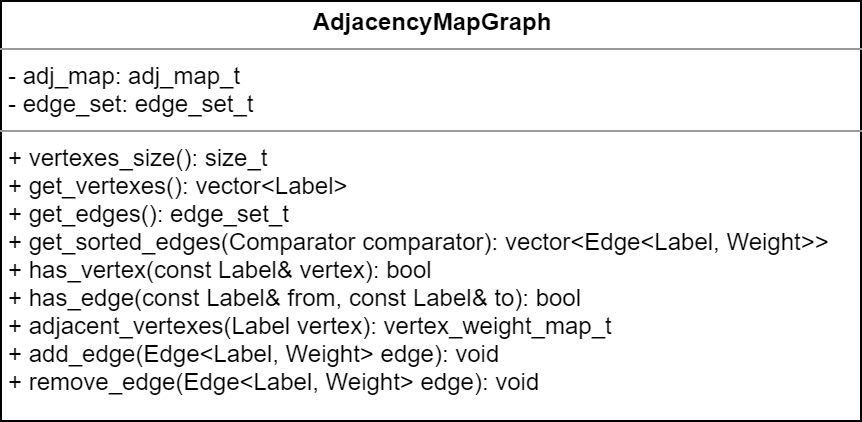
\includegraphics[width=0.7\textwidth]{./images/AdjancencyMapGrapClass.png}
	\label{fig:AdjMapGraph Class}
\end{figure}

Nella figura \ref{fig:AdjMapGraph Abstract} è riportata la trasformazione di un grafo di esempio nella relativa mappa di adiacenza che abbiamo pensato. Come è possibile notare questa mappa di adiacenza è composta da una prima mappa che elenca tutti i vertici del grafo (adj\_map\_t) e a seguire nel valore di ogni entry viene inserita una nuova mappa (vertex\_weight\_map\_t) che rappresenta gli archi del grafo: vengono elencati dunque tutti i nodi adiacenti al vertice dato con il relativo peso dell'arco. In questo modo è possibile avere tutte le operazioni di inserimento, ricerca, cancellazione e update in tempo costante, a discapito di una complessità spaziale più elevata. 

\begin{figure}[h]
	\caption{Rappresentazione della mappa di adiacenza}
	\centering
	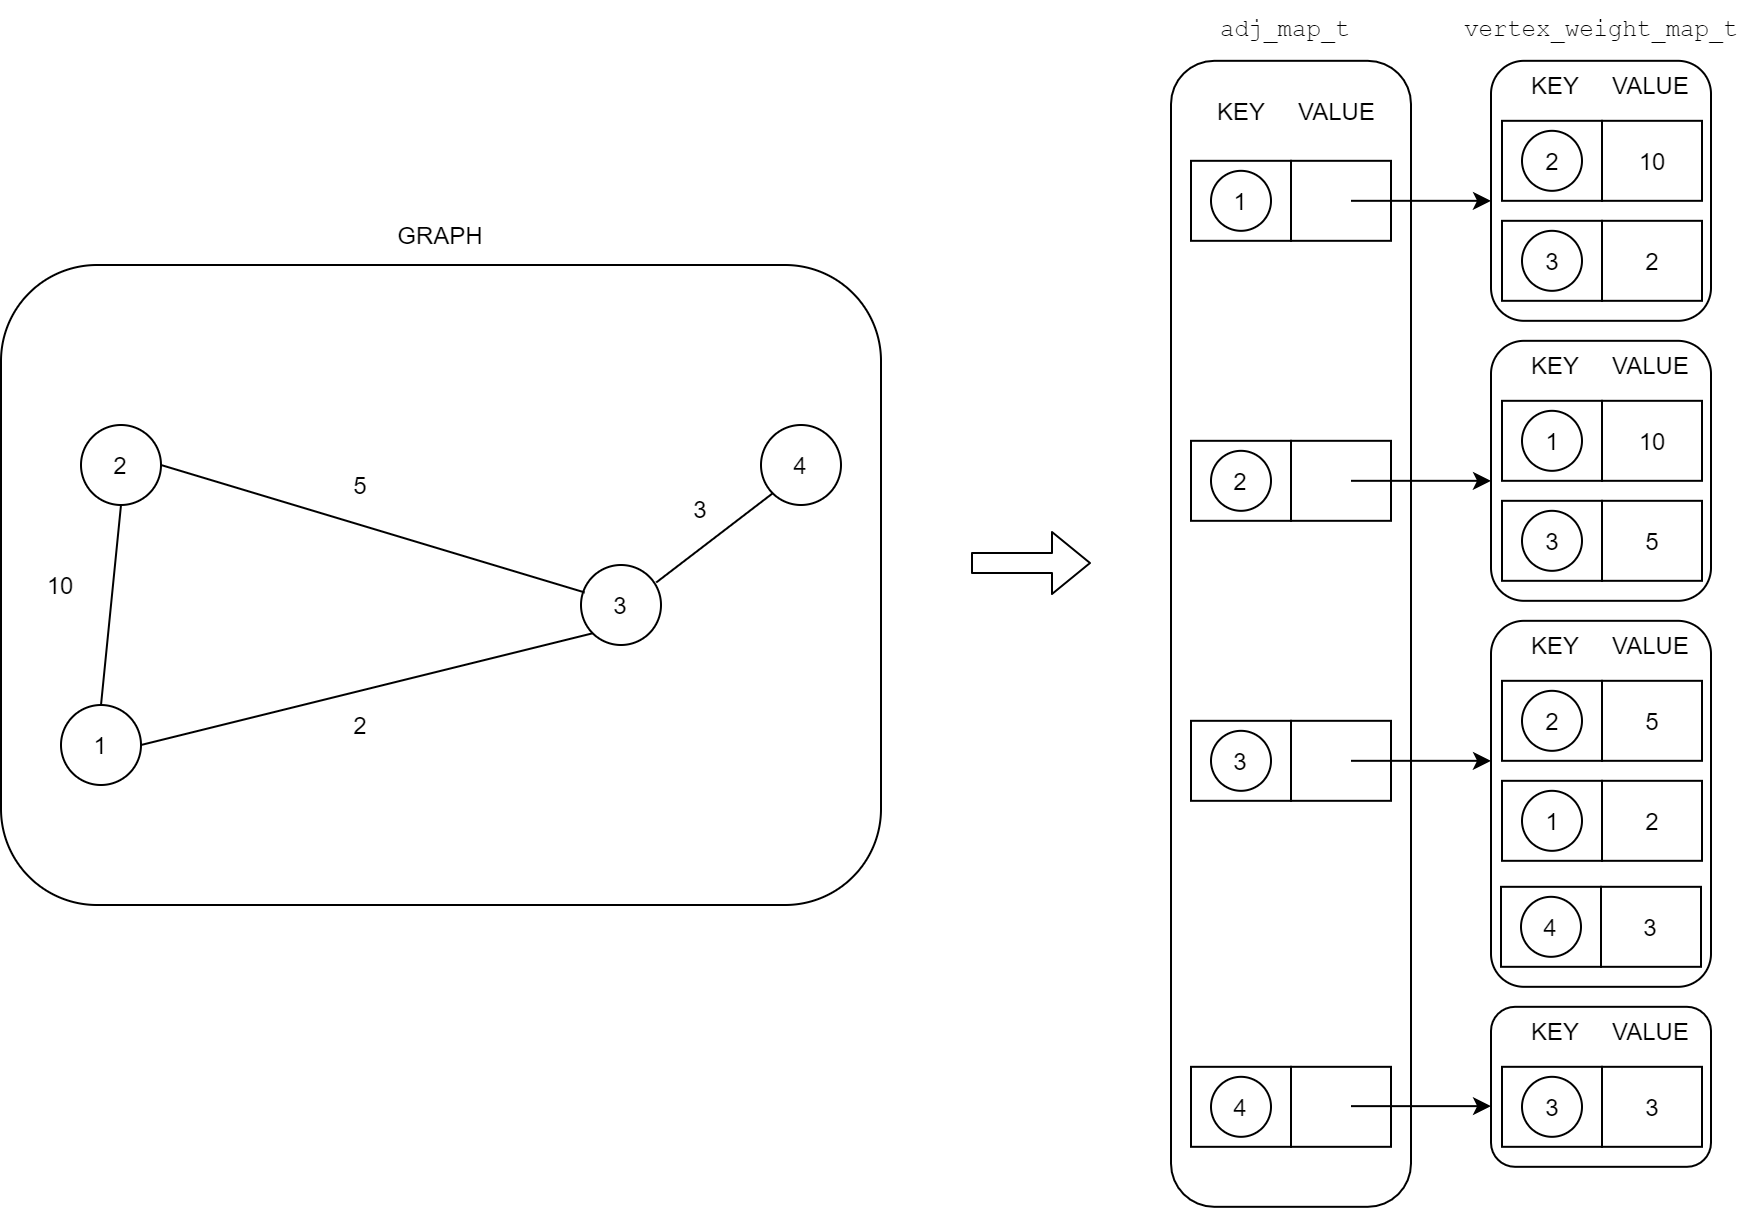
\includegraphics[width=0.7\textwidth]{./images/AdjMapGraphAbstract.png}
	\label{fig:AdjMapGraph Abstract}
\end{figure}

Nonostante la mappa di adiacenza sarebbe già stata sufficiente per salvare tutte le informazioni necessarie alla rappresentazione di un grafo, in alcune operazioni risulta essere lenta. L'esempio di operazione che ci ha spinto ad inserire una nuova struttura dati (unordered\_set in questo caso) è il metodo per ritornare tutti gli archi di un grafo in quanto tale metodo se implementato avendo a disposizione la sola mappa di adiacenza prevederebbe in maniera semplice la scansione dell'intera mappa di adiacenza, con l'inserimento degli archi via via che si incontra un nuovo vertice. Tale semplice implementazione però porterebbe alla creazione di un vettore in cui se sussiste un arco tra un vertice 2 e un vertice 3 (come nell'esempio in figura~\ref{fig:AdjMapGraph Abstract}), al vettore verrebbe aggiunto sia l'arco 2 $\rightarrow$ 3 che 3 $\rightarrow$ 2. \\

% Le cose si complicano maggiormente infatti se si restringe la richiesta di non restituire gli archi doppi come abbiamo già osservato. A tale proposito si potrebbe ricercare l'eventuale presenza di tali archi doppi ed eliminarli di conseguenza, ma il tutto richiederebbe maggiori operazioni e dunque un maggior complessità temporale.\\

% Per tali ragioni è stato deciso di affiancare alla mappa di adiacenza, un'apposita struttura dati che permettesse di tenere traccia degli archi e di avere tempi di esecuzione costanti per le operazioni di aggiunta, rimozione e ricerca. Così facendo è possibile garantire che l'operazione di restituzione degli archi singoli di un grafo abbia tempo O(m) se si richiede di restituire un vettore, o addirittura O(1) se si richiede la restituzione di un puntatore a tale struttura.

E' stato scelto dunque di utilizzare come struttura dati da affiancare unordered\_set perché oltre ad avere le caratteristiche richieste, se appositamente configurata permette di garantire l'assenza di archi doppi, compresi quelli visti nell'esempio precedente (ossia 2 $\rightarrow$ 3 e 3 $\rightarrow$ 2). Per fare ciò è stato dunque opportunamente configurato l'operatore di uguaglianza e la funzione di hash, in  modo che archi equivalenti abbiamo la stessa funzione di hash e siano riconosciuti come uguali, evitando così l'inserimento di un arco doppio visto che  unordered\_set non prevede elementi doppi al suo interno.\\

Una rappresentazione astratta di tale struttura è possibile visualizzarla nella figura~\ref{fig:edges_set}, dove è possibile notare che se viene richiesto l'inserimento di un arco 3 $\rightarrow$ 2 ove già presente un arco 2 $\rightarrow$ 3 questo non viene inserito da unordered\_set.\\

\begin{figure}[h]
	\caption{Visualizzazione astratta di edges\_set}
	\centering
	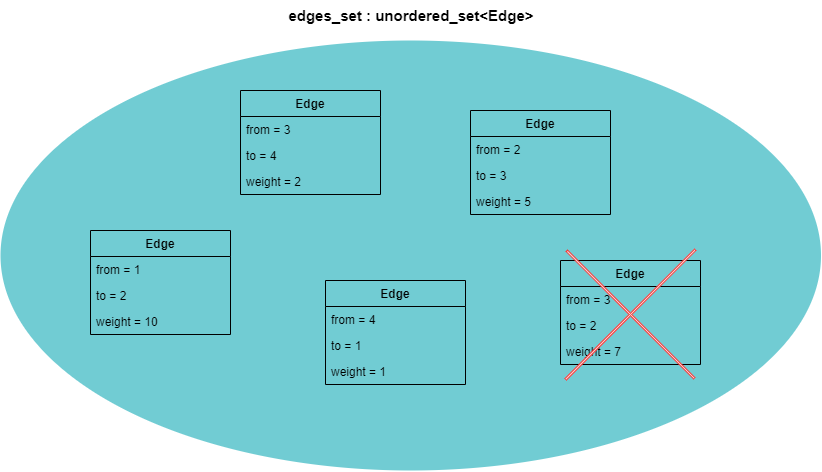
\includegraphics[width=0.7\textwidth]{./images/edges_setAbstract.png}
	\label{fig:edges_set}
\end{figure}

L'ultimo problema non ancora affrontato riguarda la possibilità di inserire un arco doppio tra due nodi uguali (come richiesto da problema), con la differenza che questi 2 archi hanno un peso diverso. Siccome la nostra implementazione non prevede la presenza di tali archi doppi, la funzione add\_eddge() si occupa di verificare l'eventuale presenza di un arco già inserito e di conseguenza i relativi pesi, per andare a modificare il peso qualora il peso del nuovo arco sia inferiore al peso dell'arco precedentemente già inserito. Per fare questo ad ogni aggiunta di un nuovo arco si va a verificare nella lista di adiacenza l'esistenza di un arco per quei due vertici:
\begin{itemize}
	\item \textbf{se l'arco era già stato aggiunto:} si confrontano i due pesi e si aggiorna il peso dell'arco solo nell'eventualità in cui il nuovo peso sia inferiore a quello già presente nella lista di adiacenza. Dopodiché se c'è stato un aggiornamento si aggiorna anche il relativo unordered\_set, eliminando l'arco precedente e si ri-aggiunge l'arco con il nuovo peso. 
	\item \textbf{se l'arco non era già stato inserito:} si inserisce l'arco sia nella lista di adiacenza che nell'unordered\_set.
\end{itemize}

\noindent Le operazioni di inserimento nei container \textit{std::unordered\_set} e \textit{std::unordered\_set} hanno complessità temporale \complexityConstant{} ammortizzata. Tuttavia, dal momento che sappiamo a priori il numero di vertici da inserire in \textit{adj\_map} e il numero di archi da inserire in \textit{edge\_set}, abbiamo preallocato un numero di bucket sufficienti ad evitare costosi \textit{rehash} in entrambi i casi.

\subsubsection {Costruzione del Grafo}

\textit{Shared/adjacency\_map\_graph\_factory.h} definisce una funzione di utilità che scorre tutte le righe del file in ingresso, salva gli archi in un vettore temporaneo, e lo trasferisce tramite \textit{move semantics} ad un nuovo oggetto di tipo \textit{AdjacencyMapGraph}. La mappa di adiacenza interpreta il grafo come spiegato nella sezione \ref{sub:graph-representation}. \\

\noindent \textbf{NOTA}: il valore dei nodi di ogni grafo è decrementato di 1 in fase di lettura del dataset di input.
Questo semplifica e rende più leggibile l'implementazione di alcune strutture dati (ad esempio i Disjoint Set) e la costruzione dell'MST con Prim.

\subsection{Strutture Dati}

Tutte le strutture dati elencate di seguito sono definite nella cartella \textit{Shared}.
Ove possibile, per la nomenclatura dei metodi abbiamo cercato di seguire lo stesso standard dei container STL di C++.
Inoltre, le strutture dati usate sono sempre preallocate in memoria quando possibile, evitando rehashing e riallocazioni dispendiose. Questo significa che la maggior parte delle operazioni indicate con \complexityConstant{} ammortizzato siano in realtà totalmente costanti nella pratica.

\subsubsection{Heap}

\textit{Heap.h} contiene la definizione astratta di una generica Heap.
Gli elementi della Heap sono salvati in un \textit{std::vector}.
Per generalizzare il concetto di MinHeap/MaxHeap, la classe usa un comparatore binario booleano. Se il funtore dato in input alla classe è
\textit{std::greater<>}, la struttura dati avrà la semantica di una Min Heap; viceversa, con il comparatore \textit{std::less<>} si avrà la semantica di una Max Heap.

\paragraph{Ottimizzazioni}\mbox{} \\

\noindent Il parametro template \textit{IsAlreadyHeap} è usato per evitare di costruire la Heap se l'utente specifica il container dato in input alla struttura dati rispetta già la proprietà di essere una Heap. Il controllo su questo flag booleano avviene a compile-time. Questa ottimizzazione garantisce un risparmio di tempo pari a \complexityN{}, ed è usata nell'implementazione dell'algoritmo di \textbf{Prim}. \\

\noindent I metodi che ripristinano la prioprietà di Heap (\textit{heapify\_up} e \textit{heapify\_down}) sono definiti in modo iterativo invece che ricorsivo, ottenendo performance migliori a parità di input. \textbf{TODO: ne siamo ancora convinti al riguardo??}

\subsubsection{Binary Heap}

\textit{BinaryHeap.h} contiene una classe concreta che eredita \textit{Heap.h} e ne implementa i metodi virtuali. Definisce una Binary Heap, ovvero è possibile rappresentare gli elementi salvati come un albero binario completo (tranne eventualmente l'ultimo livello, che potrebbe non essere completo) che rispetta la proprietà di ordinamento delle Heap.

\paragraph{Ottimizzazioni}\mbox{} \\

\noindent L'operazione di divisione per 2, necessaria per determinare ad esempio il figlio sinistro e destro di un nodo nella Heap, è stata sostituita con l'operazione di shift binario.

\subsubsection{K-ary Heap}

\textit{KHeap.h} contiene una classe concreta che eredita \textit{Heap.h} e ne implementa i metodi virtuali. Definisce una K-ary Heap, ovvero è possibile rappresentare gli elementi salvati come un albero k-ario completo (tranne eventualmente l'ultimo livello, che potrebbe non essere completo) che rispetta la proprietà di ordinamento delle Heap.
\textit{K} è un parametro template che deve essere strettamente maggiore di 2.

\subsubsection{Priority Queue}

\textit{PriorityQueue.h} è una classe concreta che eredita privatamente \textit{BinaryHeap.h} o \textit{KHeap.h}, a seconda del parametro template \textit{Heap}.
La semantica di PriorityQueue dipende dal comparatore passato al costruttore, che indica se si vuole usare una coda di priorità basata su Min Heap o su Max Heap. \\

\noindent PriorityQueue ha accesso diretto ai nodi salvati nella Heap, e usa due container associativi di tipo \textit{std::unordered\_map} per tenere traccia, ad ogni elemento della Heap, la rispettiva chiave e indice, e permetterne dunque la consultazione e l'aggiornamento in tempo costante ammortizzato. \\

\noindent Rispetto ai costruttori delle varie classi Heap, PriorityQueue richiede non un comparatore, bensì una factory di comparatori. A tale factory è data in input una mappa che associa i valori degli elementi della Heap alle rispettive chiavi. Poiché tale input è passato per reference, il comparatore generato userà sempre la versione più aggiornata della mappa.

\noindent L'operazione di aggiornamento di una chiave richiede chiavi strettamente discendenti nel caso di una MinHeap, e chiavi strettamente crescenti nel caso di una MaxHeap. Abbiamo imposto questo vincolo per mantenere la complessità di \textit{update\_key} logaritmica anziché lineare (come sarebbe se avessimo usato il metodo \textit{build\_heap} indistintamente).

\paragraph{Ottimizzazioni}\mbox{} \\

\noindent Poichè istanziare una PriorityQueue così generica e flessibile è un'operazione non banale, abbiamo creato una serie di funzioni di utilità di facile comprensione da usare. Ad esempio, per creare una coda di priorità basata su una Min Heap binaria, esiste il metodo \textit{make\_min\_priority\_queue} (analogamente esiste \textit{make\_min\_k\_priority\_queue} per Min Heap K-ari).
L'utente finale della classe non deve preoccuparsi di inserire manualmente tutti i parametri template di tali funzioni, grazie alla \textit{type deduction} di C++17.

\subsubsection{Disjoint Set}

La classe base astratta in \textit{DisjointSetBase.h} definisce il contratto dei metodi \textit{find} e \textit{unite} (il nome comunemente usato per questa operazione (\textit{union}) è una parola chiave riservata in C++).
Gli elementi sono salvati in un container \textit{std::vector} chiamato \textbf{parents}, sotto l'assunzione che gli elementi siano solo numeri interi positivi distinti numerati da $0$ a $n-1$.
Avremmo potuto rilassare questo vincolo usando una struttura dati \textit{std::unordered\_map}, ma abbiamo preferito evitare perché i vettori sono molto più performanti nella pratica. \\

È possibile rappresentare graficamente i Disjoint-Set come alberi.
\mintinline{c++}{parents[i]} indicizza il padre del nodo $i$. Al momento dell'inizializzazione della classe, ogni nodo è settato come padre di se stesso, come mostrato in figura \ref{fig:disjoint-set-base-parents}.

\begin{figure}[htbp]
	\centering
	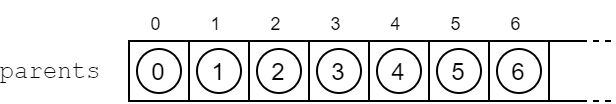
\includegraphics[width=0.7\textwidth]{./images/DisjointSetParentsVector.png}
	\caption{Inizializzazione di \textit{parents} nella classe \textit{DisjointSetBase}}
	\label{fig:disjoint-set-base-parents}
\end{figure}

\noindent Abbiamo realizzato 2 implementazioni diverse di Disjoint Set.
\textit{DisjointSet} adotta la policy \textit{union-by-size} vista a lezione, senza particolari ottimizzazioni. Definisce un membro \textit{std::vector} per salvare le dimensioni dei sottoalberi radicati nei vari nodi salvati, inizializzandolo a 1, come mostrato in figura \ref{fig:disjoint-set-sizes}.

\begin{figure}[htbp]
	\centering
    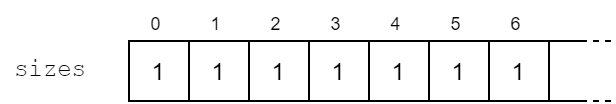
\includegraphics[width=0.7\textwidth]{./images/DisjointSetSizesVector.png}
	\caption{Inizializzazione di \textit{sizes} nella classe \textit{DisjointSet}}
	\label{fig:disjoint-set-sizes}
\end{figure}

\noindent \textit{DisjointSetCompressed}, invece, adotta la policy \textit{union-by-rank} con \textit{path-compression} tramite la tecnica \textit{path-splitting}.
Ad ogni invocazione del metodo \textit{find()} su un nodo $x$, ogni nodo nel percorso da $x$ all'antenato che identifica il set di $x$ è aggiornato per puntare al nodo "nonno". \\
\noindent DisjointSetCompressed definisce un membro \textit{std::vector} per salvare i rank dei dei vari nodi salvati, inizializzando il rank di ogni nodo a 0. Ad ogni invocazione del metodo \textit{unite()} su due nodi $x$ e $y$, ci sono due possibilità:

\begin{enumerate}
    \item Gli alberi di $x$ e $y$ hanno lo stesso rank $\rightarrow{}$ i rank del set che unirà $x$ e $y$ viene incrementato di 1;
    \item Gli alberi di $x$ e $y$ hanno rank diversi $\rightarrow{}$ il set che unirà $x$ e $y$ avrà rank pari a \\ $max\{ rank(find(x)), rank(find(y)) \}$.
\end{enumerate}

La \textit{path-compression} può modificare le altezze degli alberi ad ogni esecuzione, ma non cambierà mai il valore dei rank.
Nonostante sia possibile implementare tecniche di \textit{path-compression} anche con la policy \textit{union-by-size}, abbiamo deciso di cogliere l'opportunità di implementare la policy \textit{union-by-rank}, che non è stata spiegata a lezione. \\

In figura \ref{fig:disjoint-set-union-example} è possibile vedere un esempio di union-by-size implementato dalla classe \textit{DisjointSet}. Analogamente, in figura \ref{fig:disjoint-set-compressed-union-example} è possibile vedere un esempio di union-by-rank con path-splitting implementato dalla classe \textit{DisjointSetCompressed}.

\begin{figure}[h]
	\centering
	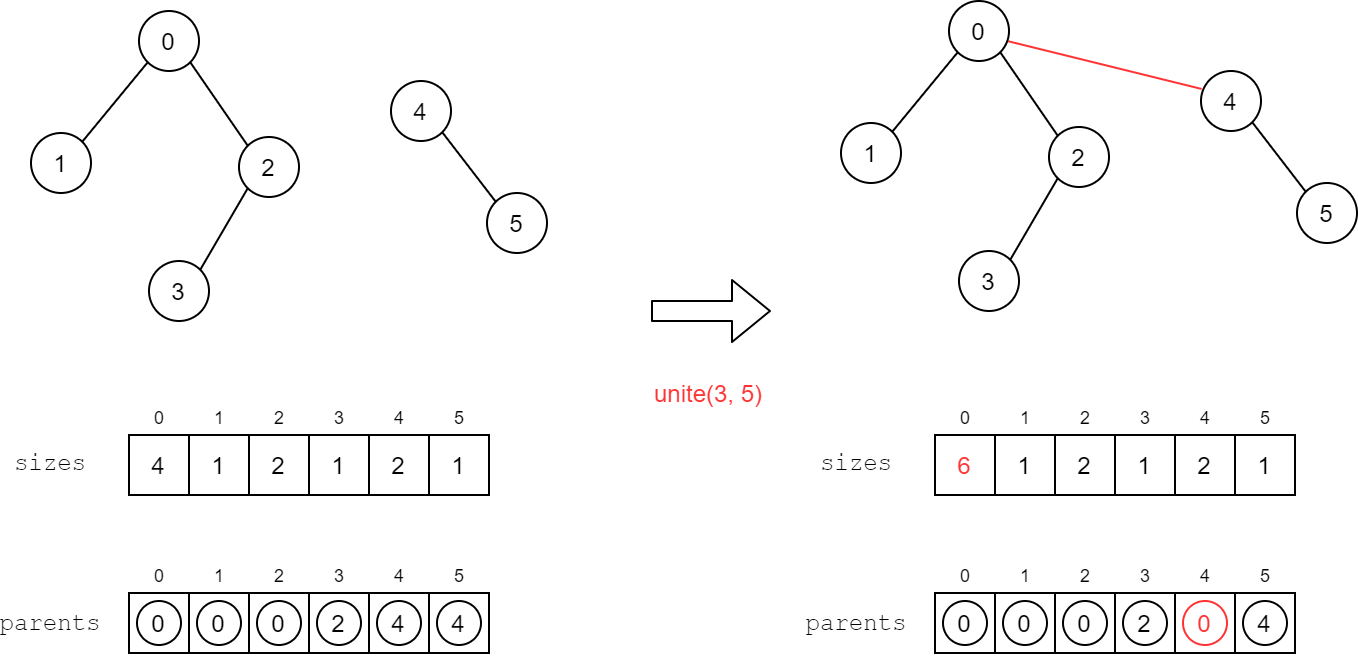
\includegraphics[width=0.7\textwidth]{./images/DisjointSetExample.png}
	\caption{Esempio di unione con DisjointSet}
	\label{fig:disjoint-set-union-example}
\end{figure}

\begin{figure}[h]
	\centering
	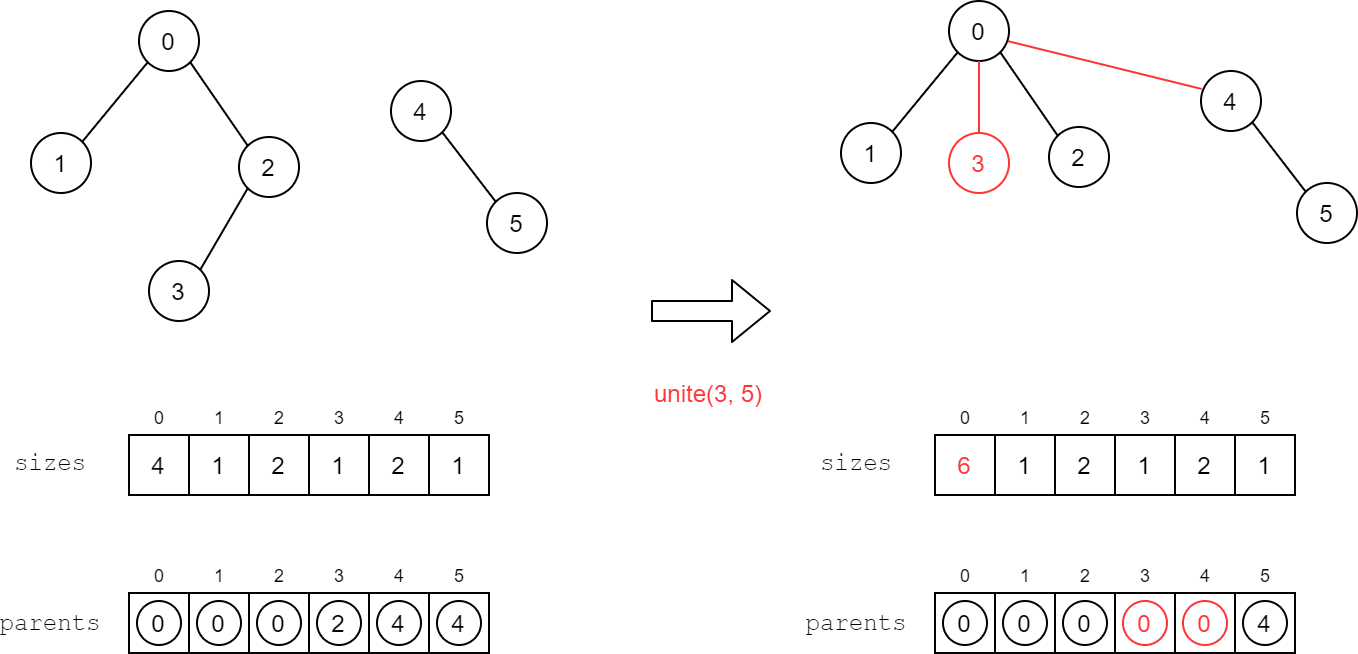
\includegraphics[width=0.7\textwidth]{./images/DisjointSetCompressedExample.png}
	\caption{Esempio di unione con DisjointSetCompressed}
	\label{fig:disjoint-set-compressed-union-example}
\end{figure}

    \newpage
    \section{Analisi delle performance}
\label{cap:performance-analysis}

\subsection{Domanda \#1}

\begin{displayquote}
Eseguite i tre algoritmi che avete implementato (Prim, Kruskal naive e Kruskal efficiente) sui grafi del dataset. Misurate i tempi di calcolo dei tre algoritmi e create un grafico che mostri la variazione dei tempi di calcolo al variare del numero di vertici nel grafo. Per ognuna delle istanze del problema, riportate il peso del minimum spanning tree ottenuto dagli algoritmi.
\end{displayquote}

\noindent Il risultato del minimum spanning tree ottenuto dagli algoritmi è illustrato dai seguenti
grafici. Le figure \ref{fig:TheThreeComparison300}, \ref{fig:TheThreeComparison1k}
e \ref{fig:TheThreeComparison2k} mostrano una comparativa piuttosto significativa tra i tre algorimti.
\'E possibile notare infatti che anche con taglie dell'input molto piccole il comportamento degli
algorimti differisce in modo cosistente: in particolare, KruskalNaive assume sin da subito un
andamento esponenziale nel numero di nodi, e non compete per nulla con KruskalUnionFind e PrimBinaryHeap.

\begin{figure}[H]
    \centering
    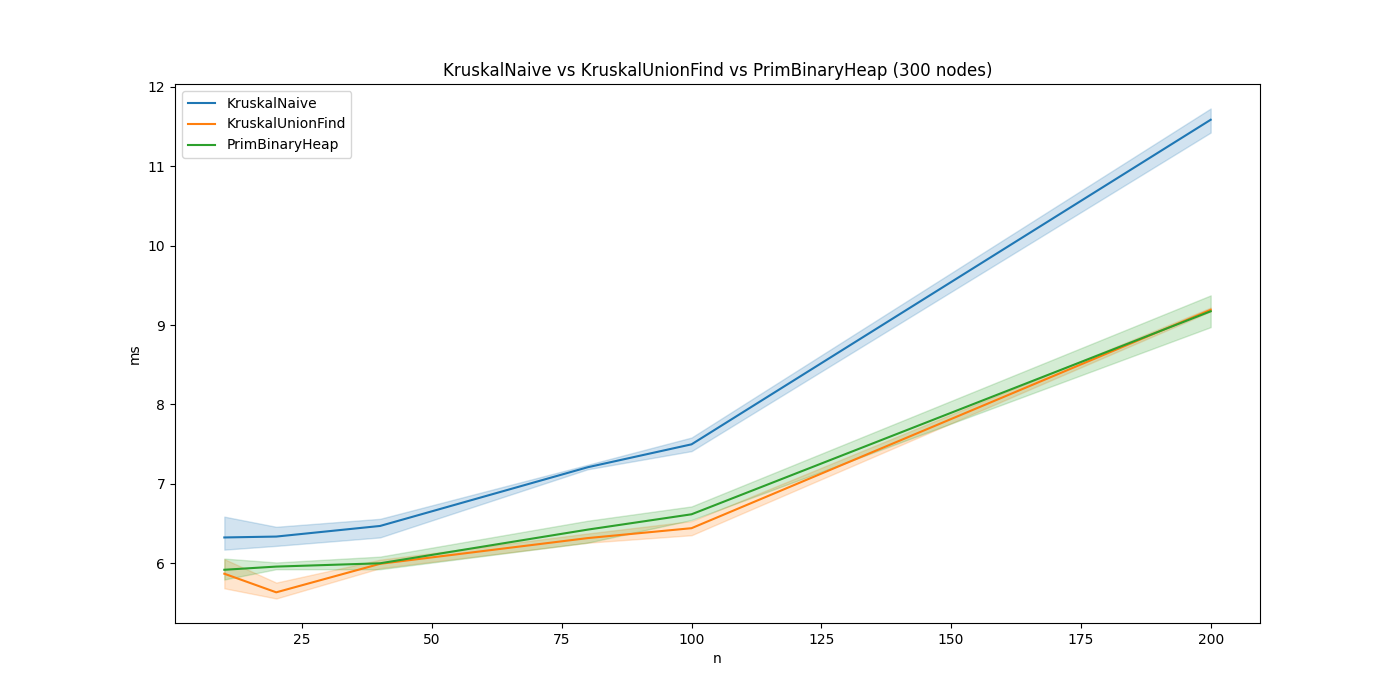
\includegraphics[width=0.9\textwidth]{./images/KruskalNaive_vs_KruskalUnionFind_vs_PrimBinaryHeap_(300_nodes).png}
	\caption{Andamento di KruskalNaive, KruskalUnionFind, PrimBinaryHeap con taglia dell'input da 0 a 300 nodi.}
    \label{fig:TheThreeComparison300}
\end{figure}

\begin{figure}[H]
    \centering
    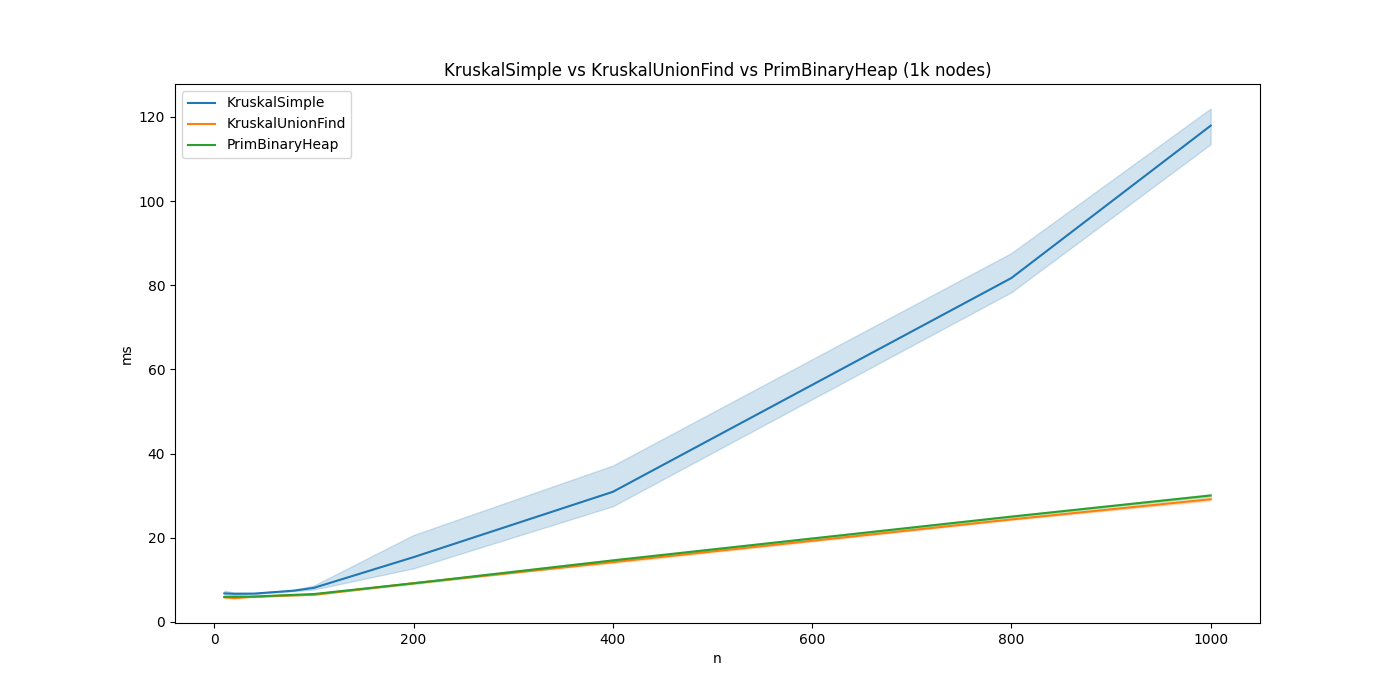
\includegraphics[width=0.9\textwidth]{./images/KruskalNaive_vs_KruskalUnionFind_vs_PrimBinaryHeap_(1k_nodes).png}
    \caption{Andamento di KruskalNaive, KruskalUnionFind, PrimBinaryHeap con taglia dell'input da 0 a 1000 nodi.}
    \label{fig:TheThreeComparison1k}
\end{figure}

\begin{figure}[H]
    \centering
    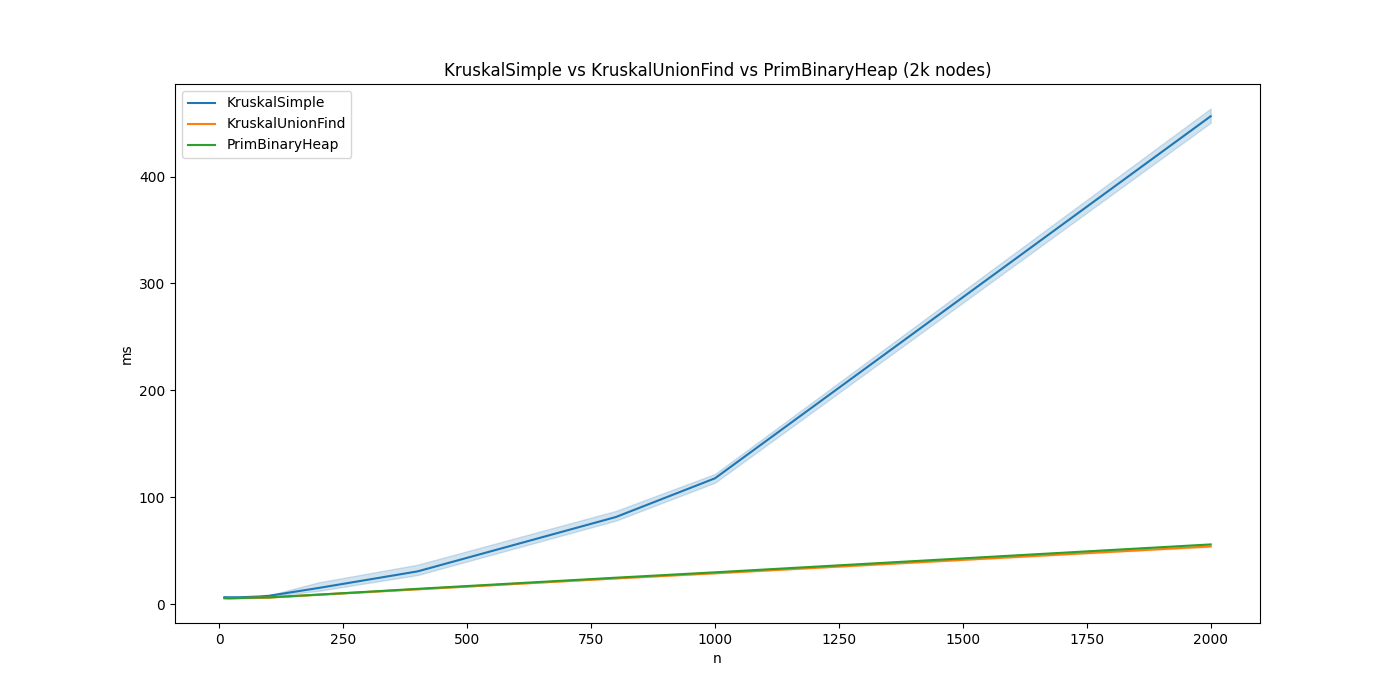
\includegraphics[width=0.9\textwidth]{./images/KruskalNaive_vs_KruskalUnionFind_vs_PrimBinaryHeap_(2k_nodes).png}
    \caption{Andamento di KruskalNaive, KruskalUnionFind, PrimBinaryHeap con taglia dell'input da 0 a 2000 nodi.}
    \label{fig:TheThreeComparison2k}
\end{figure}

\noindent Per quanto riguarda KruskalUnionFind e PrimBinaryHeap la differenza è più sottile,
e viene mostrata dalle figure \ref{fig:TheTwoComparison2k} e \ref{fig:TheTwoComparison5k}, ma è molto facile
vedere che a meno di un piccolo fattore i due hanno lo stesso trend di crescita.

\begin{figure}[H]
    \centering
    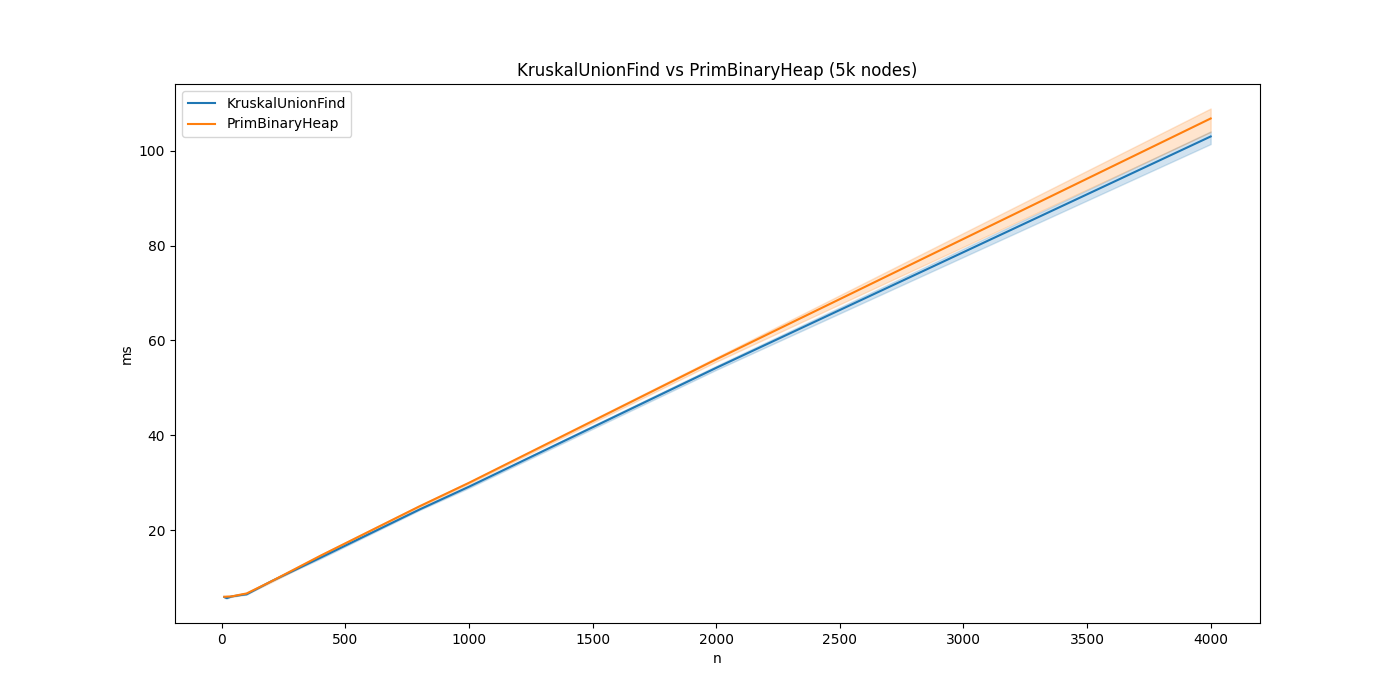
\includegraphics[width=1.0\textwidth]{./images/KruskalUnionFind_vs_PrimBinaryHeap_(5k_nodes).png}
	\caption{Andamento di KruskalUnionFind e PrimBinaryHeap con taglia dell'input da 0 a 2000 nodi.}
    \label{fig:TheTwoComparison2k}
\end{figure}

\begin{figure}[H]
    \centering
    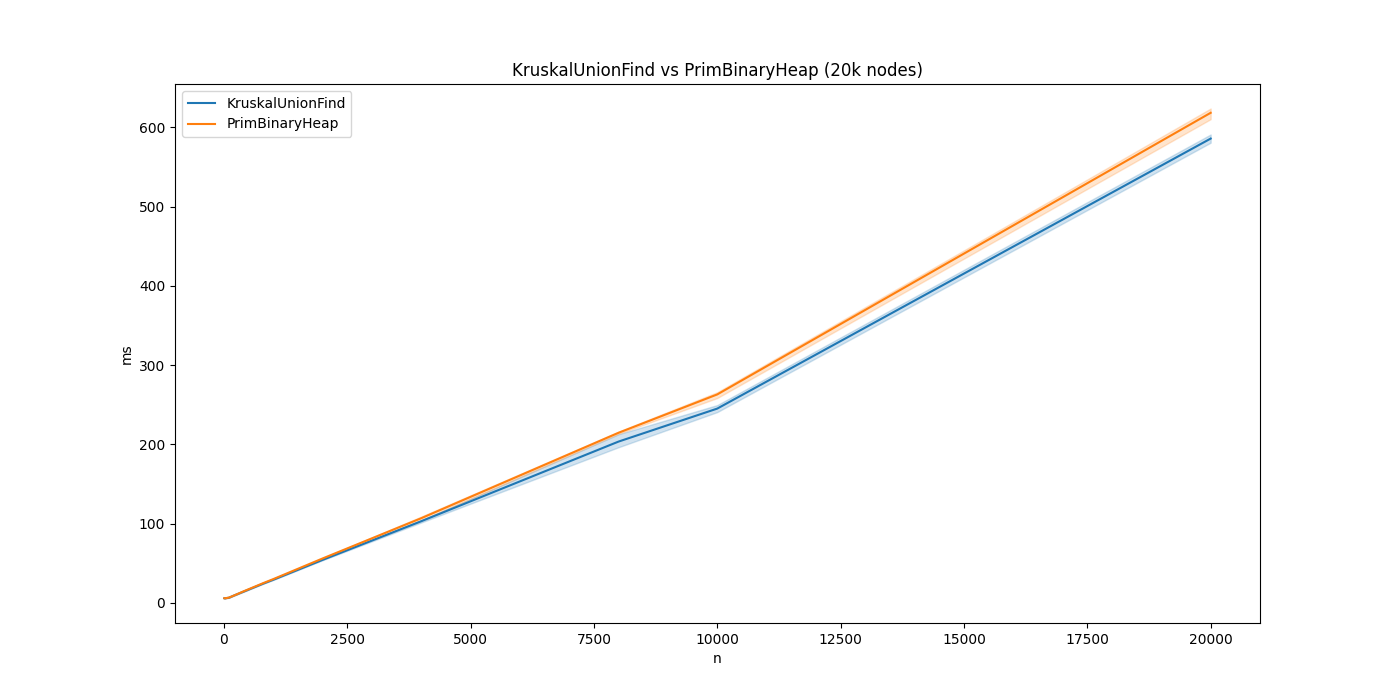
\includegraphics[width=1.0\textwidth]{./images/KruskalUnionFind_vs_PrimBinaryHeap_(20k_nodes).png}
    \caption{Andamento di KruskalUnionFind e PrimBinaryHeap con taglia dell'input da 0 a 20000 nodi.}
    \label{fig:TheTwoComparison5k}
\end{figure}

\noindent Per avere un'idea più precisa dei tempi di esecuzione degli
algorimti è possibile consultare le tabelle \ref{table:KruskalNaive-results},
 \ref{table:KruskalUnionFind-results}, \ref{table:KruskalUnionFindCompressed-results}
 e \ref{table:PrimBinaryHeap-results} in appendice \ref{cap:runtime-tables} che riportano i risultati puntuali
 dell'esecuzione degli algoritmi.

\subsection{Domanda \#2}

\begin{displayquote}
Commentate i risultati che avete ottenuto: come si comportano gli algoritmi rispetto alle varie istanze? C'è un algoritmo che riesce sempre a fare meglio degli altri? Quale dei tre algoritmi che avete implementato è più efficiente?
\end{displayquote}

\noindent Dalle tabelle di confronto \ref{table:kruskal-simple-vs-kruskal-union-find} e \ref{table:prim-binary-heap-vs-kruskal-union-find} è evidente che \textbf{KruskalUnionFind} è il più efficiente tra gli algoritmi di cui era richiesta l'implementazione. Inoltre, osservando la tabella di confronto \ref{table:kruskal-union-find-vs-kruskal-union-find-compressed}, è possibile notare che l'utilizzo della tecnica \textit{path-compression} nella struttura dati \textbf{Disjoint-Set} in realtà non abbia portato benefici, e anzi abbia peggiorato leggermente le performance (che sono comunque migliori di \textit{PrimBinaryHeap}, vedasi la tabella di confronto \ref{table:prim-binary-heap-vs-kruskal-union-find-compressed}). \\

\begin{table}[H]
\centering
    \begin{tabular}{|l|rrrrrr|}
    \hline
    &  \multicolumn{1}{c}{8k} & \multicolumn{1}{c}{10k} & \multicolumn{1}{c}{20k} & \multicolumn{1}{c}{20k} & \multicolumn{1}{c}{80k} &           \multicolumn{1}{c|}{100k} \\
    \hline
     KruskalNaive     & 7431.57  & 11939.8   & 59257     & 366313    &    1.99612e+06 &    3.12073e+06 \\
     KruskalUnionFind &  204.429 &   254.504 &   599.704 &   1249.7  & 3010.99        & 4050.49        \\ \hline
     Differenza       & 7227.15  & 11685.3   & 58657.3   & 365064    &    1.99311e+06 &    3.11668e+06 \\
     Miglioramento \%    &   97.25  &    97.87  &    98.99  &     99.66 &   99.85        &   99.87        \\
    \hline
    \end{tabular}
    \caption{Confronto tra KruskalNaive e KruskalUnionFind}
    \label{table:kruskal-simple-vs-kruskal-union-find}
\end{table}

\begin{table}[H]
\centering
    \hspace*{-1cm}
    \begin{tabular}{|l|rrrrrr|}
    \hline
    &  \multicolumn{1}{c}{8k} & \multicolumn{1}{c}{10k} & \multicolumn{1}{c}{20k} & \multicolumn{1}{c}{20k} & \multicolumn{1}{c}{80k} &           \multicolumn{1}{c|}{100k} \\
    \hline
     KruskalNaive               & 7431.57  & 11939.8   & 59257     & 366313    &    1.99612e+06 &    3.12073e+06 \\
     KruskalUnionFindCompressed &  204.429 &   256.287 &   599.704 &   1271.32 & 3062.76        & 4050.49        \\ \hline
     Differenza                 & 7227.15  & 11683.5   & 58657.3   & 365042    &    1.99306e+06 &    3.11668e+06 \\
     Miglioramento \%              &   97.25  &    97.85  &    98.99  &     99.65 &   99.85        &   99.87        \\
    \hline
    \end{tabular}
    \caption{Confronto tra KruskalNaive e KruskalUnionFindCompressed.}
    \label{table:kruskal-simple-vs-kruskal-union-find-compressed}
\end{table}

\begin{table}[H]
\centering
    \begin{tabular}{|l|rrrrrr|}
    \hline
    &  \multicolumn{1}{c}{8k} & \multicolumn{1}{c}{10k} & \multicolumn{1}{c}{20k} & \multicolumn{1}{c}{20k} & \multicolumn{1}{c}{80k} &           \multicolumn{1}{c|}{100k} \\
    \hline
     KruskalNaive   & 7431.57 & 11939.8   & 59257     & 366313    &    1.99612e+06 &    3.12073e+06 \\
     PrimBinaryHeap &  227.5  &   273.581 &   646.039 &   1365.97 & 3197.83        & 4372.45        \\ \hline
     Differenza     & 7204.07 & 11666.2   & 58610.9   & 364947    &    1.99293e+06 &    3.11636e+06 \\
     Miglioramento \%  &   96.94 &    97.71  &    98.91  &     99.63 &   99.84        &   99.86        \\
    \hline
    \end{tabular}
    \caption{Confronto tra KruskalNaive e PrimBinaryHeap.}
    \label{table:kruskal-simple-vs-prim-binary-heap}
\end{table}

\begin{table}[H]
\centering
    \hspace*{-0.25cm}
    \begin{tabular}{|l|rrrrrr|}
    \hline
    &  \multicolumn{1}{c}{8k} & \multicolumn{1}{c}{10k} & \multicolumn{1}{c}{20k} & \multicolumn{1}{c}{20k} & \multicolumn{1}{c}{80k} &           \multicolumn{1}{c|}{100k} \\
    \hline
     KruskalUnionFind           & 204.429 & 254.504 & 599.704 & 1249.7   & 3010.99  & 4050.49 \\
     KruskalUnionFindCompressed & 204.429 & 256.287 & 599.704 & 1271.32  & 3062.76  & 4050.49 \\ \hline
     Differenza                 &   0     &  -1.783 &   0     &  -21.615 &  -51.773 &    0    \\
     Miglioramento \%              &   0     &  -0.7   &   0     &   -1.73  &   -1.72  &    0    \\
    \hline
    \end{tabular}
    \caption{Confronto tra KruskalUnionFind e KruskalUnionFindCompressed.}
    \label{table:kruskal-union-find-vs-kruskal-union-find-compressed}
\end{table}

\begin{table}[H]
\centering
    \begin{tabular}{|l|rrrrrr|}
    \hline
    &  \multicolumn{1}{c}{8k} & \multicolumn{1}{c}{10k} & \multicolumn{1}{c}{20k} & \multicolumn{1}{c}{20k} & \multicolumn{1}{c}{80k} &           \multicolumn{1}{c|}{100k} \\
    \hline
     PrimBinaryHeap   & 227.5   & 273.581 & 646.039 & 1365.97  & 3197.83  & 4372.45  \\
     KruskalUnionFind & 204.429 & 254.504 & 599.704 & 1249.7   & 3010.99  & 4050.49 \\ \hline
     Differenza       &  23.071 &  19.077 &  46.335 &  116.265 &  186.843 &  321.954 \\
     Miglioramento \%    &  10.14  &   6.97  &   7.17  &    8.51  &    5.84  &    7.36  \\
    \hline
    \end{tabular}
    \caption{Confronto tra PrimBinaryHeap e KruskalUnionFind.}
    \label{table:prim-binary-heap-vs-kruskal-union-find}
\end{table}

\begin{table}[H]
\centering
    \begin{tabular}{|l|rrrrrr|}
    \hline
    &  \multicolumn{1}{c}{8k} & \multicolumn{1}{c}{10k} & \multicolumn{1}{c}{20k} & \multicolumn{1}{c}{20k} & \multicolumn{1}{c}{80k} &           \multicolumn{1}{c|}{100k} \\
    \hline
 PrimBinaryHeap             & 227.5   & 273.581 & 646.039 & 1365.97 & 3197.83 & 4372.45  \\
 KruskalUnionFindCompressed & 204.429 & 256.287 & 599.704 & 1271.32 & 3062.76 & 4050.49 \\ \hline
     Differenza                 &  23.071 &  17.294 &  46.335 &   94.65 &  135.07 &  321.954 \\
     Miglioramento \%              &  10.14  &   6.32  &   7.17  &    6.93 &    4.22 &    7.36  \\
    \hline
    \end{tabular}
    \caption{Confronto tra PrimBinaryHeap e KruskalUnionFindCompressed.}
    \label{table:prim-binary-heap-vs-kruskal-union-find-compressed}
\end{table}

% \paragraph{Premessa}\mbox{} \\

% È doveroso notare che nei dataset a disposizione non esiste alcun grafo il cui numero di archi $m$ sia maggiore del numero di vertici $n$ per più di un fattore 1.5 (ovvero, $m = $ \complexityN{}). In questo homework abbiamo quindi avuto a che fare con grafi sparsi. Poiché l'algoritmo Kruskal con Disjoint-Set ha complessità \complexityMLogN{} e

\noindent In teoria, KruskalUnionFindCompressed avrebbe dovuto essere l'algoritmo più efficiente di tutti (complessità temporale: \textbf{TODO}).
\noindent PrimBinaryHeap e KruskalUnionFind hanno la stessa complessità temporale teorica, ma in realtà la complessità delle operazioni del BinaryHeap ha un coefficiente più elevato rispetto a quelle della struttura dati Disjoint-Set. \\

\noindent Infine, data la complessità teorica di KruskalNaive (\textbf{TODO}), abbiamo ipotizzato che i tempi di calcolo nella pratica sarebbero stati più elevati a partire da grafi con poche centinaia di nodi e archi. Tale assunzione è poi stata confermata dall'analisi pratica effettuata. \\

\noindent Non abbiamo un'idea certa del perché Kruskal implementato con \textit{DisjointSetCompressed} sia meno performante di \textit{DisjointSet}. La nostra ipotesi è che, per gli input forniti al nostro programma, il \textit{cache behaviour} di KruskalUnionFind sia molto migliore di quello di KruskalUnionFindCompressed.

    \section{Test}
\label{cap:tests}

Abbiamo usato i dataset di \textit{stanford-algs} per confrontare i risultati delle nostre implementazioni degli algoritmi richiesti con gli output attesi.

\noindent Nella cartella \textit{test} sono presenti i 68 file di input e i relativi 68 file di output atteso di tali dataset. Abbiamo usato lo script Powershell \textit{test.ps1} per automatizzare il testing dei nostri programmi.

\noindent Abbiamo inoltre usato lo strumento di Continuous Integration \textit{Travis} per testare continuamente la nostra repository ad ogni push nel branch "master".

    \section{Estensioni e originalità}
\label{cap:extensions-and-originalities}

Oltre alle 3 implementazioni richieste dalla consegna dell'homework, abbiamo deciso di esplorare qualche altra estensione degli algoritmi per il calcolo del Minimum Spanning Tree visti a lezione.

\subsection{Prim con k-ary Heap}

% ...

Dal punto di vista teorico, le Fibonacci Heap hanno una complessità temporale migliore delle k-ary Heap.
Tuttavia, dal punto di vista pratico, le k-ary Heap hanno una performance migliore perché la loro struttura permette loro di sfruttare la cache locality. Inoltre le Fibonacci Heap hanno un coefficiente di complessità nascosto piuttosto elevato.
Un altro motivo per cui abbiamo deciso di non implementare le Fibonacci Heap è che sono più complesse da implementare rispetto alle k-ary Heap. \\

\noindent Quando le k-ary heap sono usate per implementare code di priorità, l'operazione di aggiornamento del valore della chiave è più veloce rispetto ad una Binary Heap (\complexityLogN{} per le Binary Heap contro \complexityLogkN{} per le k-ary Heap).
L'operazione di rimozione dell'elemento con minore chiave, tuttavia, aumenta a \complexityKLogkN{} rispetto a \complexityLogkN{} delle Binary Heap. Ma visto che nell'algoritmo di Prim le operazioni di cambio valore delle chiavi sono più comuni delle operazioni di estrazioni del minimo elemento, le k-ary Heap sono comunque più efficienti delle Binary Heap per quell'algoritmo.
% ...

\noindent Le figure \ref{fig:Prim2vsPrim4-500}, \ref{fig:Prim2vsPrim4-500} e \ref{fig:Prim2vsPrim4-80k-100k} mostrano una comparativa tra le performance
dell'algoritmo con una binary heap e un k-ary heap con $k = 4$. 
Da \ref{fig:Prim2vsPrim4-500} e \ref{fig:Prim2vsPrim4-2k-4k} si nota un lieve miglioramento delle performance utilizzando il k-ary heap, anche 
se questo comporta più uscillazione tra i tempi di runtime rispetto a input differenti. La figura \ref{fig:Prim2vsPrim4-80k-100k} invece mostra
una controtendenza tale per cui su input molto grandi il binary heap tende a fare lievemente meglio del k-ary heap.

\begin{figure}[H]
    \centering
    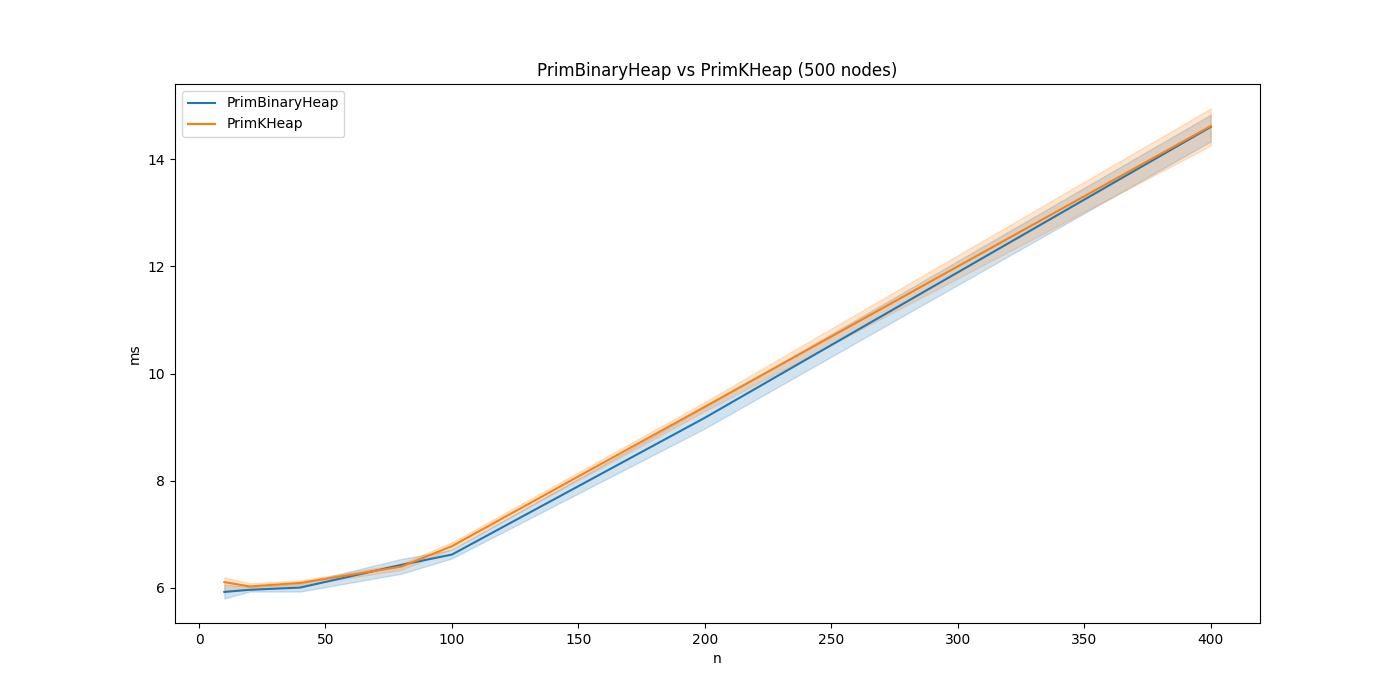
\includegraphics[width=1.0\textwidth]{./images/PrimBinaryHeap_vs_PrimKHeap_(500_nodes).png}
	\caption{Andamento di PrimBinaryHeap e PrimKaryHeap con taglia dell'input da 0 a 500 nodi.}
    \label{fig:Prim2vsPrim4-500}
\end{figure}

\begin{figure}[H]
    \centering
    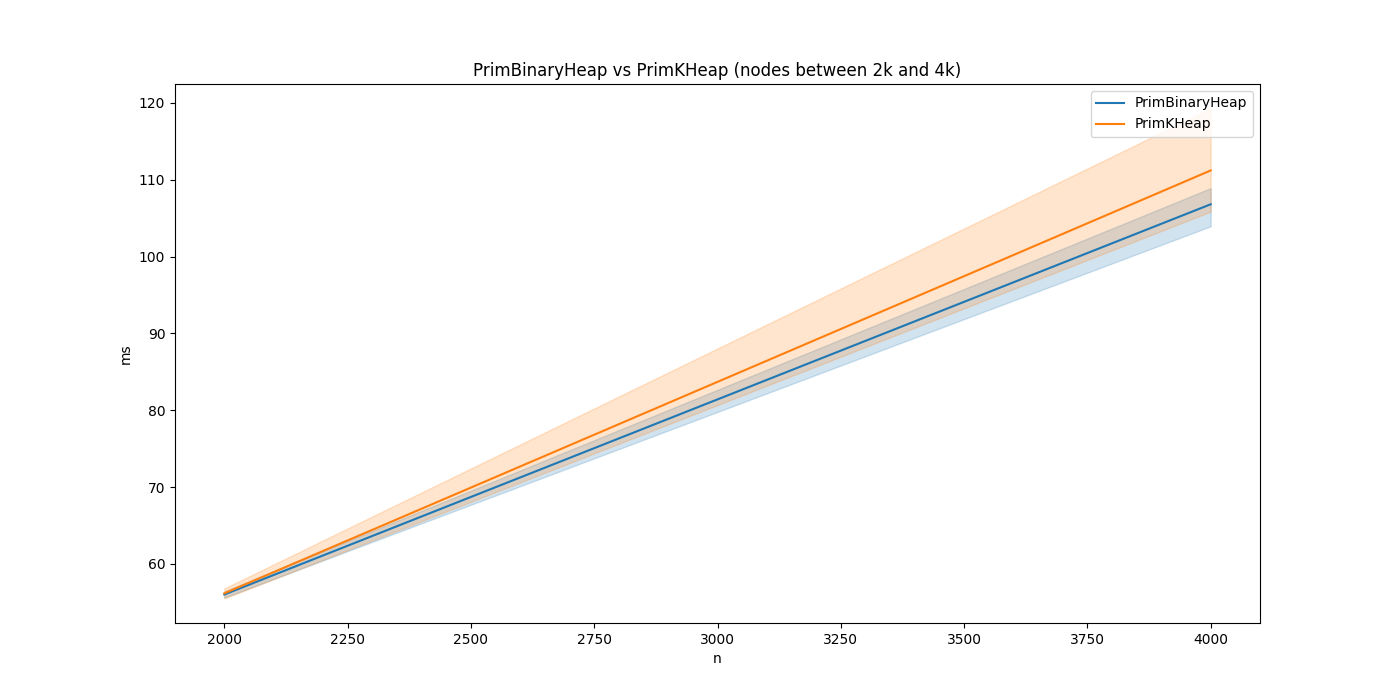
\includegraphics[width=1.0\textwidth]{./images/PrimBinaryHeap_vs_PrimKHeap_(nodes_between_2k_and_4k).png}
	\caption{Andamento di PrimBinaryHeap e PrimKaryHeap con taglia dell'input da 2k a 4k nodi.}
    \label{fig:Prim2vsPrim4-500}
\end{figure}

\begin{figure}[H]
    \centering
    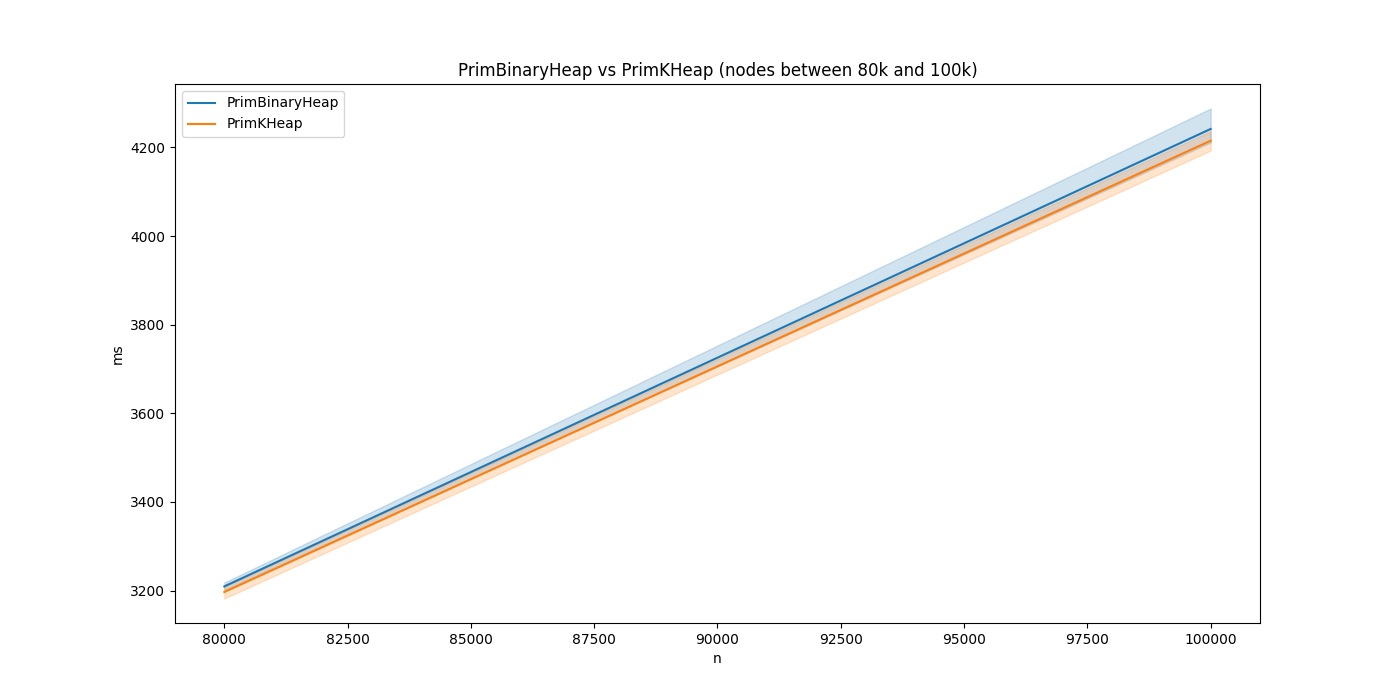
\includegraphics[width=1.0\textwidth]{./images/PrimBinaryHeap_vs_PrimKHeap_(nodes_between_80k_and_100k).png}
	\caption{Andamento di PrimBinaryHeap e PrimKaryHeap con taglia dell'input da 80k a 100k nodi.}
    \label{fig:Prim2vsPrim4-80k-100k}
\end{figure}

\subsection{Kruskal con Disjoint-Set e path-compression}

% path-compression via path-halving + union by size

    \section{Conclusioni}
\label{cap:conclusions}

In questa relazione abbiamo ampiamente gli algoritmi, le scelte implementative, i tempi di esecuzioni e i ``tricks'' usati per rendere i programmi più efficienti. \\

\noindent sezione \ref{cap:performance-analysis} abbiamo risposto alle 2 principali domande dell'homework, mentre in \ref{cap:benchmark-process} abbiamo descritto il processo di benchmark adottato, pensato per essere quanto più affidabile e stabile.
Nelle sezioni \ref{cap:code-structure}, \ref{cap:implementation-choices} e \ref{cap:algorithms} abbiamo invece discusso i dettagli tecnici, quali struttura, scelte implementative e codice degli algoritmi. \\

\noindent  La sezione \ref{cap:tests} descrive il processo di testing automatico che abbiamo adottato, che c'ha permesso di rilasciare versioni migliori degli algoritmi in più iterazioni, accorgendoci immediatamente di eventuali regressioni. La sezione \ref{cap:extensions-and-originalities} descrive infine le estensioni esplorate per soddisfare la nostra curiosità e arricchire il nostro bagaglio accademico, garantendo comunque la correttezza dei risultati. \\

\noindent L'algoritmo a cui abbiamo dedicato più tempo ed energie è, paradossalmente, KruskalNaive. Sapevamo sin dall'inizio che sarebbe stato l'algoritmo con i tempi di esecuzione più lenti, ma ci siamo ugualmente adoperati per cercare di ottimizzare l'implementazione di DFS per l'individuazione di cicli nel grafo, migliorando le performance di circa il 30\% per i grafi più complessi del dataset.

\noindent Questo progetto ci ha permesso di sperimentare più approcci, implementare e debuggare strutture dati non banali ``from scratch'' e valutare con attenzione che complessità temporali e che operazioni debba offrire una struttura dati per rendere efficienti algoritmi che la sfruttano. Questo homework ci ha permesso inoltre di migliorare la nostra comprensione del linguaggio di programmazione scelto e di come funziona la collaborazione da remoto di un piccolo team di persone. \\

\noindent Questo progetto è disponibile anche come repository pubblica su Github:

\begin{center}
\href{https://github.com/jkomyno/algorithms-hw1}{github.com/jkomyno/algorithms-hw1}
\end{center}

    % TODO: appendix with results read from CSV
  \end{document}

% https://www.latex-tutorial.com/tutorials/pgfplotstable/
